\section{Model checking}
Il \emph{model checking} è un metodo per la verifica dei sistemi. Fu introdotto da E. Clarke, A. Emerson e J. Sifakis con cui si aggiudicarono nel 2007 il A.M. Turing Award.
Il metodo del model checking è schematizzato in figura \ref{fig:model_checking}. Un \emph{model checker} riceve in \emph{input} il modello del sistema software ed i requisiti che deve soddisfare. In \emph{ouput} restituirà un valore booleano: \emph{true} o \emph{false} nel caso in cui la proprietà che si è andata a verificare  sia rispettivamente soddisfatta o non soddisfatta. Se la proprietà non è soddisfatta viene fornito un \emph{controesempio}.
\\

\begin{figure}[ht]
\begin{center}
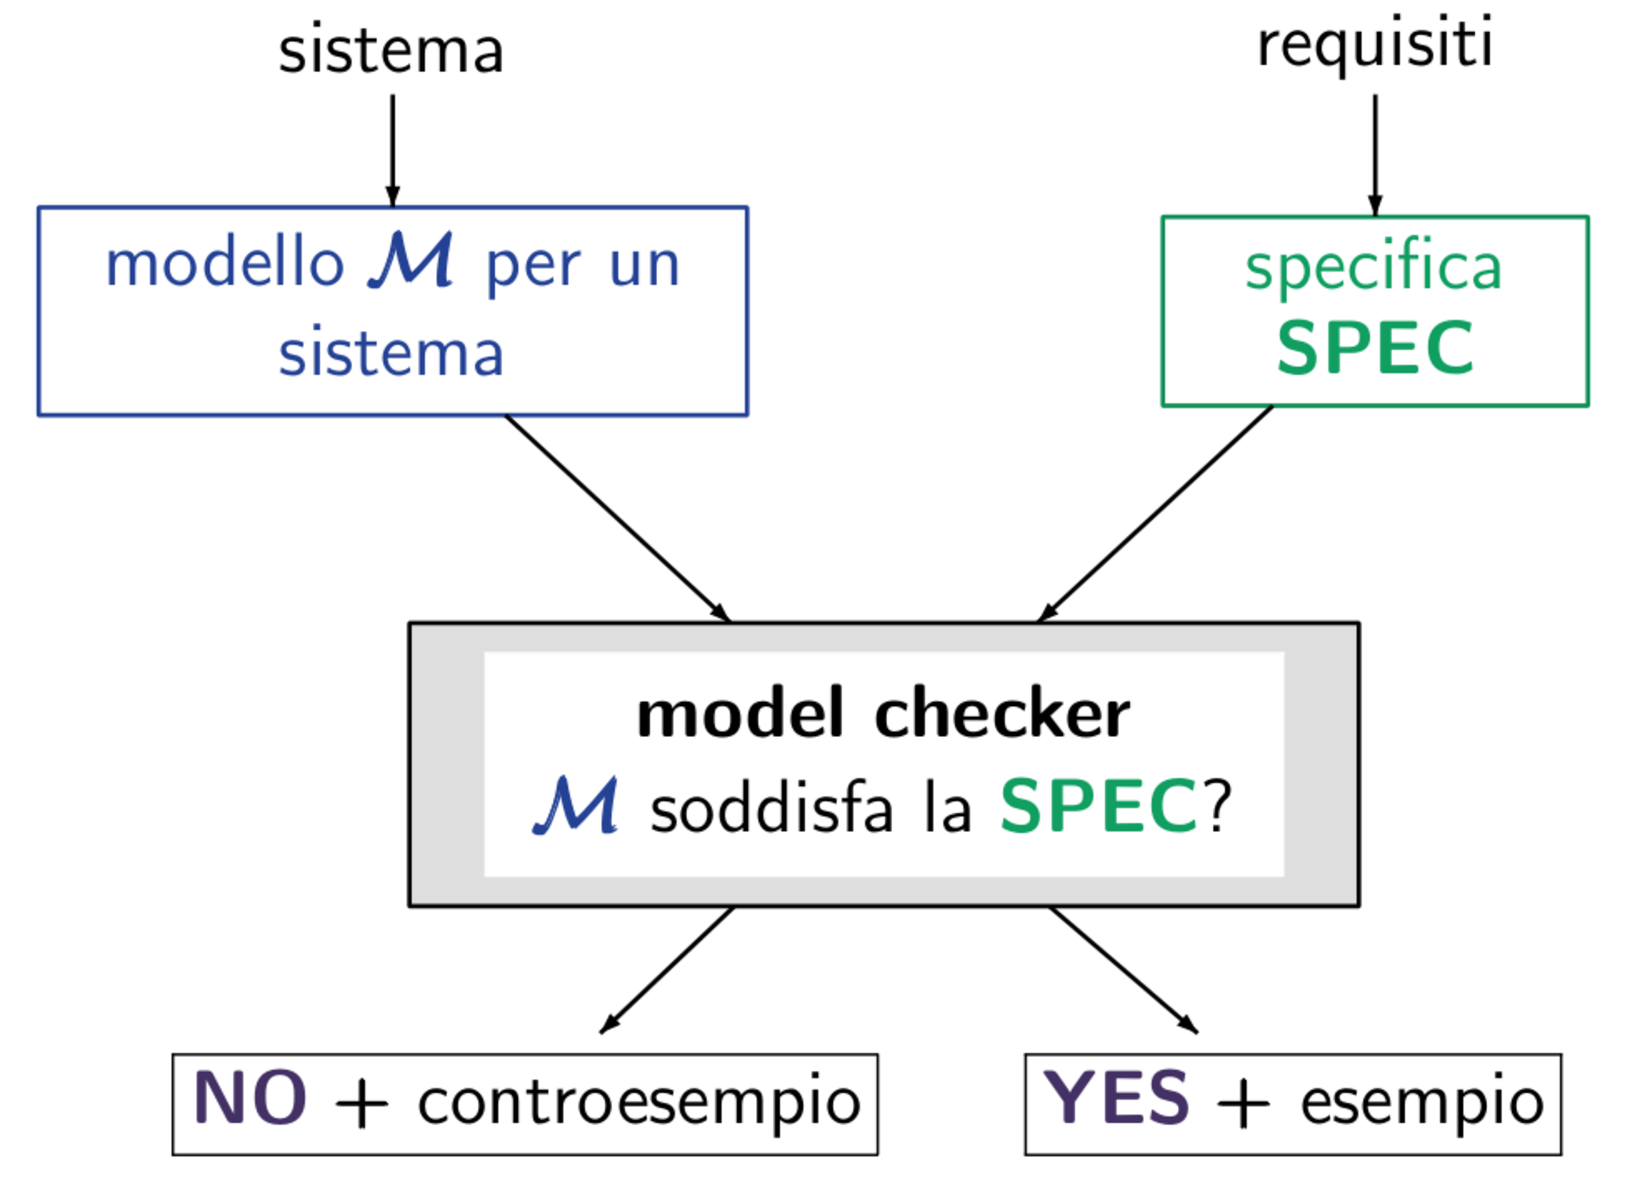
\includegraphics[scale=0.3]{img/Model-checking.pdf}
\caption{Model checking.}
\label{fig:model_checking}
\end{center}
\end{figure}

Formalmente, la verifica di una proprietà tramite model checking consiste: dato un modello del sistema $M$ con stato iniziale $s$ e data una proprietà $\phi$ che il sistema deve soddisfare, fare il model checking consiste nel dire se:

\begin{alignat}{4}
M,\ s 		& 	\models \phi \\
M,\ s  		& 	\not \models \phi
\end{alignat}

Il modello del sistema su cui vogliamo fare model checking è descritto mediante un sistema di transizione etichettato (LTS). Le proprietà da verificare sono descritte attraverso un linguaggio formale in logica temporale, nel nostro caso aCTL.

\subsection{Model checking globale e locale}

Come abbiamo detto i sistemi sono una composizione di più modelli che descrivono il comportamento di un processo. Un limite del model checking è il cosidetto fenomeno dell'\emph{esplosione dello spazio degli stati}. La rappresentazione di un sistema con un numero elevato di stati (ad esempio dell'ordine di $10^{100}$) richiede molta memoria. 

Possiamo distinguere due approcci di model checking:
\begin{itemize}
 \item model checking globale
 \item model checking locale
\end{itemize}

Il \emph{model checking globale}, consiste nell'andare a verificare se tutti gli stati del sistema preso in considerazione, verificano una proprietà. Questa è un'operazione computazionalmente onerosa in quanto verrà generato l'intero spazio degli stati. Inoltre, vengono generati anche gli stati che non sono rilevanti al fine di dimostrare la soddisfacibilità della formula. 
L'approccio utilizzato è quello di una ricerca \textit{bottom-up} a partire dalle foglie dell'albero fino a risalire alla radice.

Viceversa, il \emph{model checking locale} genera solo gli stati che servono effettivamente a verificare la proprietà. In questo caso viene adottato un approccio \textit{top-down}, e cioè a partire da un nodo radice si percorre l'albero verso le foglie.

\clearpage
\subsubsection{Existential normal form (ENF)}

Al fine di sviluppare un model checker, viene utilizzata una notazione alternativa alle formule aCTL, l'Existential Normal Form (ENF), che permette una più semplice trasposizione in forma algoritmica.
Qualsiasi formula aCTL può essere infatti scritta come combinazione delle formule ENF.

\begin{equation}
\Phi ::= true \; | \; ap \; | \; \Phi_1 \wedge \Phi_2 |  \neg \Phi | \exists \; \chi_A \; \Phi \; | \; \exists ({\Phi_1}_A \; \mathcal{U}\; \Phi_2) \; | \; \exists ({\Phi_1}_A \; \mathcal{U}_B \; \Phi_2) \; | \; \exists \Box_A \Phi
\end{equation}

I passi da eseguire per verificare se uno stato, appartenente a TS,  verifica una formula aCTL $\hat{\Phi}$, sono i seguenti:

\begin{enumerate}
\item si converte la formula $\hat{\Phi}$ nella sua equivalente $\Phi$ in ENF
\item si calcola ricorsivamente l'insieme $ Sat(\Phi) = \lbrace s \in S | s \models \Phi \rbrace $
\item TS, $s_i \; \models \Phi $ se e solo se $ s_i \in Sat(\Phi) $
\end{enumerate}

\clearpage

Definiamo quindi per casi, i possibili valori assumibili da Sat($\Phi$):

\begin{alignat}{4}
Sat(true)					&\quad 	\rightarrow	\quad&&	S 	\\
Sat(ap)					&\quad	 \rightarrow	\quad&&	\lbrace s | ap \in L(s) \rbrace 	\\
Sat(\Phi \wedge \Psi)			&\quad	 \rightarrow	\quad&&	Sat(\Phi) \cap Sat(\Psi)  	\\
Sat(\neg \Phi)				&\quad	 \rightarrow	\quad&&	S \ Sat(\Phi) 	\\
Sat(\exists \mathcal{X}_A \Phi)		&\quad	 \rightarrow	\quad&&	\lbrace s | Post_A(s) \cap Sat(\Phi) \neq \emptyset 	\\
Sat(\exists \Phi_A \mathcal{U} \Psi)	&\quad	 \rightarrow	\quad&	\begin{split} & \text{il più piccolo sottoinsieme T} \subseteq \text{S,tale che:} 	\\
														& 1)\; Sat(\Psi) \subseteq T  \\
														& 2)\; se \;s \in Sat(\Phi) \wedge Post_A(s) \cap T \neq \emptyset \Rightarrow s \in T
												\end{split} \\
Sat(\exists \Phi_A \mathcal{U}_B \Psi)	&\quad	 \rightarrow	\quad&	\begin{split} & \text{il più piccolo sottoinsieme T} \subseteq \text{S,tale che:} 	\\
														& 1)\; se \; s \in Sat(\Phi) \wedge Post_B(s) \cap Sat(\Psi) \neq \emptyset \Rightarrow s \in T \\
														& 2)\; se \; s \in Sat(\Phi) \wedge Post_A(s) \cap T \neq \emptyset \Rightarrow s \in T
												\end{split} \\
Sat(\exists \Box_A \Phi)			&\quad	 \rightarrow	\quad&	\begin{split} & \text{il più piccolo sottoinsieme T} \subseteq \text{S,tale che:} 	\\
														& 1)\; Sat(\Psi) \subseteq T  \\
														& 2)\; se \; s \in T \Rightarrow Post_A(s) \cap T \neq \emptyset 
												\end{split}
\end{alignat}



